% !TeX spellcheck = en_US
\documentclass[AMbeamer%               style
               ,optEnglish%            language
               %,handout%               deactivate animation
               ,optBibtex%              bibliography tool
               %,optBiber%               bibliography tool
               ,optBibstyleAlphabetic%
               ,optBeamerClassicFormat% 4:3 format
               %,optBeamerWideFormat%   16:9 format
               %,optExzellenz%
               ]{AMlatex}%
\setbeameroption{show notes on second screen}% show notes}% Show all notes
%
%
% Tikz libraries
\usepackage{standalone}%
\usetikzlibrary{angles, arrows.meta, backgrounds, calc, decorations.pathmorphing, shapes.geometric, patterns, positioning, timeline, quotes}%
%
% Glossaries
\usepackage[acronyms, toc]{glossaries}
\makenoidxglossaries
\loadglsentries{source/glossary.tex} % important update for glossaries, before document
%
% Set paths
\graphicspath{{figures/}}%
\addbibresource{source/literature.bib}%
%
% Set meta data
% -------------
\title[Comparison of Controllers for Trunk Stabilization in a Bipedal Robot]{Comparison of Controllers for Trunk Stabilization in a Bipedal Robot}%
\def\PresentationType{\AMlangGerEng{Auftaktvortrag}{Initial Presentation}}%
%\def\PresentationType{\AMlangGerEng{Abschlussvortrag}{Final Presentation}}%
%\def\PresentationThesisType{\AMlangBachelorsThesis}%
%\def\PresentationThesisType{\AMlangSemesterThesis}%
\def\PresentationThesisType{\AMlangMastersThesis}%
%\def\PresentationThesisType{\AMlangInterdisciplinaryProject}%
\author[F. Schausberger]{Felix Schausberger}%
\def\PresentationExaminer{\AMnamesProfRixen}%
\def\PresentationSupervisor{Dr.-Ing. Daniel Renjewski}%
\date{\AMutilsDate{11}{10}{2022}}%%
%
% Setup of header and footer
\AMbeamerSetupHeader{\AMlayoutHeaderCustomChair}%
\AMbeamerSetupFooterCD%
%
\begin{document}%
%
% Start with titlepage
\AMbeamerTitlePageStudentThesis%
%
%
\begin{frame}{Problem description}%
    \begin{columns}[T,onlytextwidth]%
        \begin{column}[T]{0.48\textwidth}%
            Balancing the trunk on long legs is a major challenge in bipedal walking.\\
            Task Description:
            \begin{enumerate}
                \item Quantify and analyze different trunk pitch control strategies.
                \item Implement relevant controllers in JenaFox simulation.
                \item Evaluate selected approaches on robotic test environment.
            \end{enumerate}%
        \end{column}%
        \begin{column}[T]{0.48\textwidth}%
            \begin{figure}[htb]%
                \centering%
                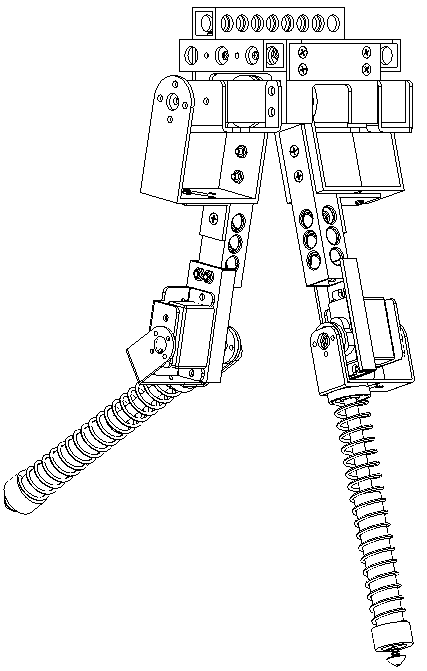
\includegraphics[width=0.5\textwidth]{figures/jena-fox-wireframe-transparent-black.png}%
                \caption{JenaFox Bipedal Walking Robot.}%
                \label{fig:jenafox}%
            \end{figure}%
        \end{column}%
    \end{columns}%
\end{frame}%
%
\note[itemize]{%
    \item Bipedal walking: Complex task, highly dynamical gait that involves flight phase, during which no force can be applied to environment
    \item Among others, one of the biggest challenges: balance torso on long legs
    \item Analyze, implement, evaluate (JenaFox on left)
}%
%%
\begin{frame}{Objective of the Thesis}%
    \begin{columns}[T,onlytextwidth]%
        \begin{column}[T]{0.48\textwidth}%
            \begin{enumerate}
                \item Starting point:\\Stiff spring limits rotation of trunk
                \item Approach:\\Gradually reduce spring while adjusting controller
                \begin{itemize}
                    % \item Intuitive~\cite{Raibert1986}
                    \item \textbf{Collision based}~\cite{Lee2011}
                    \item \acrshort{h-slip}~\cite{Shen2012}
                    \item Virtual Pivot Point (VPP)~\cite{Maus2008}~\cite{Maus2010}
                \end{itemize}
                \item Objective:\\Free rotation without restrictions
                % \item Note: Friction still simulated, but not as a spring
            \end{enumerate}
        \end{column}%
        \begin{column}[T]{0.48\textwidth}%
            \begin{figure}[htb]%
                \centering%
                \includestandalone{figures/objective/objective}%
                \caption{Overview of the selected methods to achieve the goal from the current state of the project.}%
                \label{fig:objective}%
            \end{figure}%
        \end{column}%
    \end{columns}%
\end{frame}%
%
\note[itemize]{% 
    \item David Lee and others, premise: Discrete footfalls prevent consistent orthogonal relationship between force and velocity vectors, thus kinetic energy is lost as GRF performs mechanical work at \acrshort{com}
    \item Extension of canonical \acrshort{slip} with constant hip torque and linear leg damping during stance called \acrfull{h-slip}
    \item \acrshort{vpp}, a fixed point on the torso above the \acrshort{com}, where \acrshort{grf} are directed to via hip torque
    \item Overall objective: Get rid of spring and enable a free rotation of the trunk without restrictions
    \item Note: Friction still included, just not as spring
}%
%%
\begin{frame}{Comparison criteria}%
    \begin{columns}[T,onlytextwidth]%
        \begin{column}[T]{0.48\textwidth}%
            \begin{itemize}
                \item Maximum allowable perturbation~\cite{Rummel2008}~\cite{Maus2010}
                    \begin{itemize}
                        \item Limit cycle: $\upsilon_{n + 1} = \upsilon_n$
                        \item Poincaré map: $\upsilon_{n + 1} = S(\upsilon)$
                    \end{itemize}
                \item Disturbance response % recovery process of the model after a disturbance: how fast the model returns to a limit cycle.
                \item Mechanical cost analysis
            \end{itemize}
            Possible disturbances:
            \begin{itemize}
                \item Horizontal velocity $\dot{x}_0$ % (instantaneous speed increase/decrease of the \acrshort{com})
                \item Floor height $\dot{y}_0$
                \item Torso angular rate $\dot{\phi}_0$
            \end{itemize}
        \end{column}%
        \begin{column}[T]{0.48\textwidth}%
            \begin{figure}[htb]%
                \centering%
                \includestandalone{figures/disturbance-rejection/disturbance-rejection}%
                \caption{Determination of the maximum allowable disturbance rejection. (Adapted from~\cite{Bommel2011}, p. 5)}%
                \label{fig:disturbance-rejection}%
            \end{figure}%
        \end{column}%
    \end{columns}%
\end{frame}%
%
\note[itemize]{%
    \item Disturbance rejection: maximum allowable perturbation of model
    \item First, limit cycle, which model is in when initial states remain unchanged for consecutive strides, will get determined
    \item Important role: Poincaré (Púokaré) map: Mapping between initial states of consecutive strides
    \item Explain model
    \item Other possible comparison criteria: Disturbance response: Recovery process of model after disturbance,  mechanical cost analysis
    \item Possible disturbances: $x_0$, $y_0$, $\phi_0$: Introduced as single error on initial state of limit cycle
}%
%
% (Bommel, 2011): The initial conditions define the set of state parameters for which the running model is in limit cycle, which means the runner is in a nominally periodic, stable sequence of hops. The initial state of a consecutive hop is determined by the end state of the previous hop. The mapping between the initial states of consecutive hops is called a Poincaré map.
%
% The model is in limit cycle when the initial states remain unchanged for consecutive hops
%
% limit cycle is found by minimising the difference between the initial state v0 and the state of the running model after one step v1
%
% Disturbances are introduced to the model as a single error on the initial state of the limit cycle.%
\begin{frame}{Work Plan and necessary Resources}%
    Tools:
    \begin{itemize}
        \item Controller implementation and simulation in MATLAB\textsuperscript{\tiny\textregistered} and Simulink\textsuperscript{\tiny\textregistered} (2022a)
            \begin{itemize}
                \item Version Control System (git via \href{https://gitlab.lrz.de/}{gitlab})
            \end{itemize}%
        \item Documentation and scientific discussion in Visual Studio Code with \LaTeX
            \begin{itemize}
                \item Version Control System (git via \href{https://codeberg.org/fesch/master-thesis}{codeberg})
                \item Citation and reference management with JabRef
            \end{itemize}%
    \end{itemize}%
\end{frame}%
%%
\begin{frame}{Time schedule}%
    \begin{figure}[htb]%
        \centering%
        \includestandalone{figures/schedule/schedule}%
        \caption{Intended schedule of the master thesis.}%
        \label{fig:schedule}%
    \end{figure}%
\end{frame}%
%%
\begin{frame}{Summary}%
    \begin{columns}[T,onlytextwidth]%
        \begin{column}[T]{0.48\textwidth}%
            Balancing the trunk on long legs is a major challenge in bipedal walking.\\
            Task Description:
            \begin{enumerate}
                \item Quantify and analyze different trunk pitch control strategies.
                \item Implement relevant controllers in JenaFox simulation.
                \item Evaluate selected approaches on robotic test environment.
            \end{enumerate}%
        \end{column}%
        \begin{column}[T]{0.48\textwidth}%
            \begin{figure}[htb]%
                \centering%
                \includestandalone{figures/objective/objective}%
                \caption{Overview of the selected methods to achieve the goal from the current state of the project.}%
                \label{fig:objective}%
            \end{figure}%
        \end{column}%
    \end{columns}%
\end{frame}%
%%
%
% End with titlepage
\AMbeamerTitlePageStudentThesis%
%
% Appendix
\begin{frame}[fragile=singleslide]{Collision based approach}% [shrink=20]
    \shorthandoff{"} % Needed for quotes
    \begin{columns}[T,onlytextwidth]%
        \begin{column}[T]{0.48\textwidth}%
            \begin{itemize}
                \item If $F \perp V$: No collision occurs
                \item Discrete footfalls: $F \not\perp V$: Kinetic energy is lost~\cite{Biewener2018}
                % Discrete footfalls preclude a consistent perpendicular relationship~\cite{Biewener2018}
                % \item Kinetic energy is lost as ground reaction force does mechanical work on centre of mass ($CoM$)
                % \item Quantified: Mechanical cost of transport ($CoT_{mech}$)
            \end{itemize}%
            Key advantages:~\cite{Lee2013}
            \begin{itemize}
                \item \acrfull{com} dynamics get considered in every instance of contact during stride
                \item Dimensionless % , allowing comparisons across species of vastly different size and comparisons across gravity conditions
                \item Independent of a priori models % of \acrshort{com} mechanics applies equally to any gait
                \item Explains the mechanical \acrfull{cot} from first principles
            \end{itemize}%
        \end{column}%
        \begin{column}[T]{0.48\textwidth}%
            \begin{figure}[htb]%
                \centering%
                \includestandalone{figures/collision-based-approach/collision-based-approach}%
                \caption{Schematic representation of the collision based approach. Shown are the force vector $F$ and velocity vector $V$ with their corresponding angles, $\theta$ and $\lambda$. The collision angle $\phi$ is the deviation of the orthogonal relation between $F$ and $V$. (Adapted from~\cite{Lee2011}, p. 4)}%
                \label{fig:collision-based-approach}%
            \end{figure}%
        \end{column}%
    \end{columns}%
\end{frame}%
%
\note[itemize]{%
    \item Mechanics: Modeled in terms of “inelastic” collisions by limb with ground
    \item If $F \perp V$: No collision occurs: No work done at \acrshort{com},~\eg wheel without rim but infinite spokes
    \item Intermittent foot contacts during legged locomotion result in relatively abrupt, collision-like changes in \acrshort{com} direction, which require mechanical work
    \item Dimensionless, allowing comparisons across species of vastly different size and comparisons across gravity conditions
    \item Independent of a priori models of \acrshort{com} mechanics: applies equally to any gait
}%
%
%
\begin{frame}{\acrfull{h-slip}}%
    % \begin{columns}[T,onlytextwidth]%
    %     \begin{column}[T]{0.48\textwidth}%
            \begin{itemize}
                \item Extension of canonical \acrfull{slip} with constant hip torque and linear leg damping during stance
                \item Closer to a realistic robot design than \acrshort{slip}% SLIP: energy conserving
                \item \acrshort{slip}: Partially asymptotically stable~\cite{Seyfarth2002} % Although it can return to periodic locomotion when subjected to a perturbation in velocity direction [15], it cannot stabilize the system energy.
                \item \acrshort{h-slip}: Full asymptotic stability of \acrshort{com} locomotion~\cite{Shen2012}
            \end{itemize}%
    %     \end{column}%
    %     \begin{column}[T]{0.48\textwidth}%
    %         %
    %     \end{column}%
    % \end{columns}%
\end{frame}%
%
\note[itemize]{%
    \item \acrshort{slip}: energy conserving: Although it can return to periodic locomotion when subjected to perturbation in velocity direction, it cannot stabilize system energy
}%
%%
\begin{frame}{\acrfull{vpp}}%
    \begin{columns}[T,onlytextwidth]%
        \begin{column}[T]{0.48\textwidth}%
            \begin{itemize}
                \item Takes leg orientation into account % In contrast to a conventional PD controller
                \item If the \acrshort{vpp} is aligned with the leg, no torso torque is applied and the resulting \acrfull{grf} is directed at the hip joint. (left)
                \item When the torso is tilted backwards, a negative torso torque must be applied to align the \acrshort{grf} with the \acrshort{vpp}. (right) % The torso torque results in an additional GRF at the foot, denoted by F_T . The spring force F_S and the torso torque F_T combine to a resultant GRF, denoted by F, directed at the VPP.
            \end{itemize}%
        \end{column}%
        \begin{column}[T]{0.48\textwidth}%
            \begin{figure}[htb]%
                \centering%
                \includestandalone{figures/virtual-pivot-point/virtual-pivot-point}%
                \caption{Schematic representation of the \acrshort{vpp}, a fixed point on the torso above the \acrshort{com}, where the \acrshortpl{grf} are directed via a hip torque. (Adapted from~\cite{Maus2010}, p. 3)}%
                \label{fig:virtual-pivot-point}%
            \end{figure}%
        \end{column}%
    \end{columns}%
\end{frame}%
%
\note[itemize]{%
    \item When \acrshort{grf} always directs at \acrshort{vpp}: becomes virtual hinge around which the torso will rotate
    \item Transforms difficult task of balancing inverted pendulum to system consisting of pendulum suspended from hinge, which is intrinsically stable
}%
% 
% (Bommel, 2011): When the GRF always directs at the VPP, the VPP becomes a virtual hinge around which the torso will rotate. Essentially, this transforms the difficult task of balancing an inverted pendulum to a system consisting of a pendulum suspended from a hinge, which is intrinsically stable.
%
% (Bommel, 2011): The controller can exert a torso torque only during the stance phase, since no GRF are present during the flight phase.
%%
%
% References
\AMbeamerSetFooterText{References}%
\begin{frame}[allowframebreaks]{References}%
    %\sloppy% "Word"-like typesetting in order to improve breaking lines with long URLs/DOIs
    \printbibliography[heading=none]%
\end{frame}%
%%
%
% Glossary
\AMbeamerSetFooterText{Glossary}%
\begin{frame}[allowframebreaks]{Glossary}%
    \printnoidxglossaries%
\end{frame}%
%
\end{document}%
%
%
